\setchapterpreamble[u]{\margintoc}
\chapter{A Brief Introduction}
\labch{intro}


\section{What We Talk About When We Talk About Urbit}
\labsec{urbittalk}

Urbit is a functional-as-in-language, network-first, compatibility-breaking
operation function (or hosted operating system).  But what does any of this mean?  As we explore Urbit software development throughout this book, keep in mind that every piece of Urbit aims to solve a ambitious battery of critical problems with the existing legacy World Wide Web.

The Urbit project intends to cut the Gordian knot of user autonomy and privacy.  To this end, the Urbit developers have articulated an approach prioritizing \emph{a legible future-proof program stack}, \emph{data security}, and \emph{cryptographic ownership}.  The ambitious scope of this project—and the evolution of the goals over the decade of the 2010s—has led many to have difficulty grasping what exactly Urbit is all about.

\subsection{A Series of Unfortunate Events}

\paragraph{Centralization}.  For most contemporary corporations, whether enterprise-scale or startup, the driving factor for growth and revenue became the number of customers (users) they were able to attract to their platform or app.  Services like \texttt{del.icio.us} (founded 2003) and Flickr (founded 2004) betokened a wave of massive centralization, cemented by Facebook, Google, and Apple in the late aughts.  TODO XXX number of users on each in 2010

As users jostled onto burgeoning social media platforms, their patterns of behavior changed, and more and more social interactions of significance took place within "walled gardens," service platforms that interfaced only poorly with the exterior web.  Vendor lock-in and the nonportability of user data between platforms meant that consumer choice became a byword.  It became (and remains) difficult for any user to find out just what a corporation or even an app knows about them, particularly given the rise of surveilling cookies and data trackers.

The shift to mobile computing starting with the 2007 launch of Apple's iPhone drove a rise in cloud computing and cloud storage.  To many users, the data storage and access permissions on their data became largely illegible.  Sometimes this led to poor assumptions, such as that the custodial corporation would never allow a leak, or that the data would always be backed up safely.  As projects failed (like \texttt{del.icio.us}) or unilaterally changed policies (Tumblr), users permanently lost data.  Given the effort involved in curating tags, bookmarks, images, contacts, and research data, these outcomes frequently amounted in the loss of years of human effort.

\paragraph{Data leaks}.  During the 2000s and 2010s, data leaks became so common as to hardly merit notice.  As users flocked to corporate platforms for social media, publishing, photography, dating, and every other aspect of digital life, insufficient attention was given by corporations to both the practical security of user data and the potential fallout of leaks.  Data breaches grew in number ever year, and affected corporations of every size in every industry.

\begin{itemize}
  \item  2013:  Evernote, 50 million records
  \item  2014:  Ebay, 145 million records
  \item  2015:  Ashley Madison, 32 million records
  \item  2016:  Yahoo!, 1 billion records
  \item  2017:  Experian, 147 million records
  \item  2019:  Facebook, 850 million records
  \item  2019:  CapitalOne, 106 million records
\end{itemize}

("Records" does not equal "people" or even "accounts," of course, rendering these numbers mutually incommensurable.  Regardless, the scale staggers the mind.)  Sometimes these breaches were the result of clever social engineering; more frequently, someone forgot to properly salt password hashes or just stored or transmitted them in unencrypted plaintext.  Occasionally, the data were even just left available at a deprecated or forgotten API endpoint.  Identity security is challenging to get right, and those who had custody of user data were frequently subject to moral hazard.
%Data are from [Juliana de Groot, "The History of Data Breaches"](https://digitalguardian.com/blog/history-data-breaches) and [Wikipedia, "List of Data Breaches"](https://en.wikipedia.org/wiki/List_of_data_breaches).

\paragraph{The looming software stack}.  A combination of practical manufacturing limits ending Moore's law and a complexifying operating system and software stack led to a long-term stagnation in the perceived speed and fluidity of user experience with computers.  For the most part, even as multicore CPUs become more widespread, software bloat grows more acute with each new operating system version.  For many enterprise developers, there have been insufficient incentives to simplify software rather than to continue making it more complex.  Minimalist software by and large remained the demesne of hackers and code golf enthusiasts.

For instance,
TODO MS Word menu structure

Even websites with visually minimalist aesthetics often presented
\citeauthor{Ceglowski2015}
a
- Optional Reading: [Maciej Cegłowski, "The Website Obesity Crisis"](https://idlewords.com/talks/website_obesity.htm)
- Optional Reading: [Maciej Cegłowski, "Build a Better Monster: Morality, Machine Learning, and Mass Surveillance"](https://idlewords.com/talks/build_a_better_monster.htm)
- Optional Reading: [Mark Tarver, "The Cathedral and the Bizarre"](http://marktarver.com/thecathedralandthebizarre.html)


\paragraph{Security breaches}.



heartbleed

\paragraph{Morbidity in open-source software projects}.

FOSS lanternfish


\paragraph{Spam}.

We have a cascading stack of legacy software and strange interdependencies.  We have an anemic FOSS program in general.  Taken together, actually getting the functionality you want as a user often requires a proprietary platform anyway.


For the Urbit developers, "security" means both guaranteed cryptographic ownership and access, and \emph{security against future utilization} or future-proofing.

Data ownership

Urbit is a  network-first,
compatibility-breaking

As of this writing, Urbit runs on any of several interpreters as a "hosted OS," or a

% Write like SeeTee shareholder letter but for Urbit, demolish all objections

Let us posit a social operating system, or SOS;  a protocol for network-oriented platforms to utilize to ensure that user requirements are met securely.  If we enumerate user-oriented desiderata for a social operating system, surely the following must rank prominently:

\begin{itemize}
	\item  Privacy
	\item  Security
	\item  Ownership
\end{itemize}



The Urbit project does not completely solve all of these problems—for instance, pwned hardware—but it offers a reasonable set of solutions for many of the social and software issues raised by contemporary corporate practice on the World Wide Web.


\section{Azimuth, the Urbit Address Space}
\labsec{azimuth}



In \citeyear{Zooko2001}, digital cash pioneer Zooko Wilcox-O'Hearn postulated that a namespace cannot simultaneously possess three qualities:

\begin{enumerate}
	\item  distributedness ("in the sense that there is no central authority which can control the namespace, which is the same as saying that the namespace spans trust boundaries"),
	\item  security ("in the sense that name lookups cannot be forced to return incorrect values by an attacker, where the definition of "incorrect" is determined by some universal policy of name ownership"), and
	\item  human legibility (or interpretable by human users).

This trilemma, dubbed Zooko's triangle, laid down a challenge to cryptographic researchers, who spent some effort to empirically refute the postulate.

In the case of Urbit,

% https://web.archive.org/web/20011020191610/http://zooko.com/distnames.html


Many modern printed textbooks have adopted a layout with prominent
margins where small figures, tables, remarks and just about everything
else can be displayed. Arguably, this layout helps to organise the
	discussion by separating the main text from the ancillary material,
	which at the same time is very close to the point in the text where
	it is referenced.

This document does not aim to be an apology of wide margins, for there
are many better suited authors for this task; the purpose of all these
words is just to fill the space so that the reader can see how a book
written with the kaobook class looks like. Meanwhile, I shall also try
to illustrate the features of the class.

The main ideas behind kaobook come from this
\href{https://3d.bk.tudelft.nl/ken/en/2016/04/17/a-1.5-column-layout-in-latex.html}{blog
	post}, and actually the name of the class is dedicated to the author
of the post, Ken Arroyo Ohori, which has kindly allowed me to create a
class based on his thesis. Therefore, if you want to know more reasons
to prefer a 1.5-column layout for your books, be sure to read his blog
post.

Another source of inspiration, as you may have noticed, is the
\href{https://github.com/Tufte-LaTeX/tufte-latex}{Tufte-Latex Class}.
The fact that the design is similar is due to the fact that it is very
difficult to improve something wich is already so good. However, I like
to think that this class is more flexible than Tufte-Latex. For
instance, I have tried to use only standard packages and to implement as
little as possible from scratch;\sidenote{This also means that
understanding and contributing to the class development is made easier.
Indeed, many things still need to be improved, so if you are interested,
check out the repository on github!} therefore, it should be pretty easy
to customise anything, provided that you read the documentation of the
package that provides that feature.

\marginnote[2mm]{In addition to the pronounceable \patp s, the sigil system affords a unique visual representation of each addressable point less than $2^{32}$.}

In this book I shall illustrate the main features of the class and
provide information about how to use and change things. Let us get
started.

\section{Accessing Urbit}
\labsec{access}

The \Class{kaobook} class focuses more about the document structure than
about the style. Indeed, it is a well-known \LaTeX\xspace principle that
structure and style should be separated as much as possible (see also
\vrefsec{doesnot}). This means that this class will only provide
commands, environments and in general, the opportunity to do things,
which the user may or may not use. Actually, some stylistic matters are
embedded in the class, but the user is able to customise them with ease.

The main features are the following:

\begin{description}
	\item[Page Layout] The text width is reduced to improve readability
	and make space for the margins, where any sort of elements can be
	displayed.
	\item[Chapter Headings] As opposed to Tufte-Latex, we provide a
	variety of chapter headings among which to choose; examples will be
	seen in later chapters.
	\item[Page Headers] They span the whole page, margins included, and,
	in twoside mode, display alternatively the chapter and the section
	name.\sidenote[][-2mm]{This is another departure from Tufte's
	design.}
	\item[Matters] The commands \Command{frontmatter},
	\Command{mainmatter} and \Command{backmatter} have been redefined in
	order to have automatically wide margins in the main matter, and
	narrow margins in the front and back matters. However, the page
	style can be changed at any moment, even in the middle of the
	document.
	\item[Margin text] We provide commands \Command{sidenote} and
	\Command{marginnote} to put text in the
	margins.\sidenote[][-2mm]{Sidenotes (like this!) are numbered while
	marginnotes are not}
	\item[Margin figs/tabs] A couple of useful environments is
	\Environment{marginfigure} and \Environment{margintable}, which, not
	surprisingly, allow you to put figures and tables in the margins
	(\cfr \reffig{marginmonalisa}).
	\item[Margin toc] Finally, since we have wide margins, why don't add
	a little table of contents in them? See \Command{margintoc} for
	that.
	\item[Hyperref] \Package{hyperref} is loaded and by default we try
	to add bookmarks in a sensible way; in particular, the bookmarks
	levels are automatically reset at \Command{appendix} and
	\Command{backmatter}. Moreover, we also provide a small package to
	ease the hyperreferencing of other parts of the text.
	\item[Bibliography] We want the reader to be able to know what has
	been cited without having to go to the end of the document every
	time, so citations go in the margins as well as at the end, as in
	Tufte-Latex. Unlike that class, however, you are free to customise
	the citations as you wish.
\end{description}

\begin{marginfigure}[-5.5cm]
	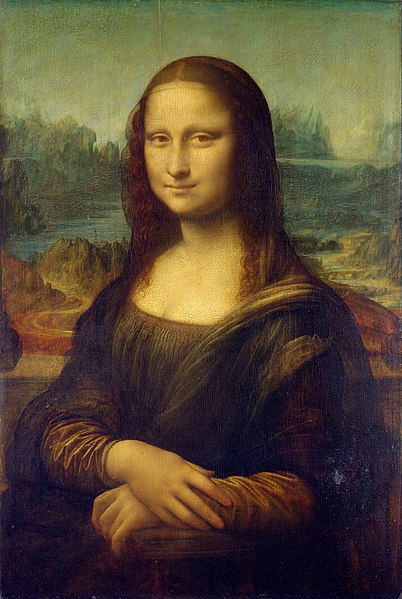
\includegraphics{monalisa}
	\caption[Sigils]{Some sigils\\
	\url{https://media.urbit.org/site/posts/essays/help-the-environment.jpg}}
	\labfig{marginsigils}
\end{marginfigure}

\section{Developing for Urbit}
\labsec{developing}

Urbit development can be divided into three cases:

\begin{enumerate}
	\item  Kernel development
	\item  Userspace development, Urbit-side (\gall~and generators)
	\item  Userspace development, client-side (Urbit API)
\end{enumerate}

This guide focuses on getting the reader up to speed on the second development case early, then branches out.

We encourage the reader to approach each example and exercise in the following spirit:

\begin{enumerate}
  \item  Identify the input and outputs, preferably at the data type level and contents.
	\item  Reason analogically from other Hoon examples available in the text and elsewhere.
	\item  Create and complete an outline of the code content.
	\item  Devise and compose a suitable test suite.
\end{enumerate}
